\section{Introduction}

\subsection{Cross-DC Erasure Coding: Why Now?}

As the entire IT industry is rapidly moving to the cloud, more and more data
centers are being built all over the globe. The event that one of the data
centers will fail catastrophically becomes inevitable over time. In other words,
this is no longer a matter of ``if'', but rather ``when''. {\em Designing for
  disasters}~\cite{keeton04designing} becomes essential and data stored in the
cloud have to be protected against catastrophic data center failure.

There have been a long line of prior work~\cite{oceanstore:asplos00,
  pond:fast13, hail:ccs09, racs:socc10, hu12nccloud} arguing for storing data
objects in erasure coded form, as opposed to replication, across geo-graphically
distributed data centers. Compared to geo-replication, cross-DC erasure coding
tolerates data center failure and ensures durability, while significantly
reduces storage cost. The same economic force that has driven cloud providers to
erasure code data within individual data centers naturally extends to the
cross-DC scenario.

Nevertheless, none of the cloud providers today offer options to erasure code
customer data across data centers. This is largely due to the prohibitive cost
of cross-DC network traffic. The reduction in storage cost comes at the
additional cost of inflated cross-DC network traffic, for both read/write during
normal operation and access/rebuild in the event of data center failure, as
discussed in detail in Section~\ref{sec:motivation}. Since the total cost of
storing customer data includes both the storage and the cross-DC network
traffic, cross-DC erasure coding has not become an economic option yet.

\begin{table}[thp]
\centering
\small
\begin{tabular}{|l|c|c|}
\hline
TransAtlantic Cable             & FLAG Atlantic 1~\cite{bib:FA-1}   & MAREA~\cite{bib:MAREA1, bib:MAREA2}
\\ \hline \hline
Ready For Service               & 2001                              & 2017
\\ \hline
Cost (Billion)                  & 1.1                               & undisclosed
\\ \hline
Capacity                        & 10 Gbps                           & 160 Tbps
\\ \hline \hline
\end{tabular}
\caption{Cross-DC bandwidth cost reducing by orders of magnitude.}
\label{tab:mears}
\end{table}

Fortunately, the technology advancement in wide area networking has progressed
to a point where new innovations have greatly reduced cross-DC bandwidth cost.
There are two key driving forces. 1) The erbium-doped fiber
amplifiers~\cite{mears1986low} make it practical to amplify a huge spectrum of
optical signal directly, without the need to first convert to electrical signal.
2) Dense Wave Division Multiplexing (DWDM) is in turn enabled by the fiber
amplifiers, which can send 10+ terabits per second over single fiber~\cite{zhu2011112}.

Most recently, Facebook and Microsoft have teamed up to build $MAREA$, a new
fiber optic cable under the Atlantic Ocean that uses eight pairs of fiber optic
strands and will come online in 2017 with 160 Tbps capacity~\cite{bib:MAREA1,
  bib:MAREA2}. Compared to MAREA, FLAG Atlantic 1~\cite{bib:FA-1}, another
transatlantic cable came online in 2001, had a mere capacity of 10 Gbps. The
over 10,000$\times$ bandwidth increase in less than two decades is summarized in
Table~\ref{tab:mears}. While the cost of MAREA remains undisclosed, it suffices
to say that the cross-DC bandwidth cost has reduced by several orders of
magnitude. Indeed, the significant cost reduction in cross-DC bandwidth is now
making cross-DC erasure coding economically attractive.
% And Project Giza addresses technical challenges so as to make such economical solution a reality.

\comment{bib:MAREA1, http://www.wsj.com/articles/facebook-and-microsoft-to-build-fiber-optic-cable-across-atlantic-1464298853}
\comment{bib:MAREA2, http://www.usatoday.com/story/experience/2016/05/26/microsoft-facebook-undersea-cable-google-marea-amazon/84984882/}
\comment{bib:FA-1, https://en.wikipedia.org/wiki/Fiber-Optic_Link_Around_the_Globe}

\subsection{Giza Overview}

Project Giza addresses key technical challenges so as to turn cross-DC erasure
coding from an economically attractive proposal to a practically sound reality.
It designs and implements an externally consistent
(linearizable~\cite{herlihy90linearizability}), versioned object store that
erasure codes objects across global datacenters.
%Giza provides an externally consistent (linearizable~\cite{herlihy1990linearizability}) versioned cloud storage service, which erasure codes data objects and stores them across globally distributed data centers.

Customers access Giza by creating Giza storage accounts. For each storage
account, Giza allows the customers to specify the set of data centers where
their data are striped across. In addition, the customers have the flexibility
to choose an erasure coding scheme. Giza employs classic $n = k + m$
Reed-Solomon coding, which generates $m$ parity fragments from $k$ data
fragments. All $n$ fragments are stored in different data centers, where 1)
failures of up to $m$ arbitrary data centers are tolerated; and 2) data can be
reconstructed from any $k$ out of the $n$ data centers. By allowing the
customers to specify the set of data centers and choose the erasure coding
scheme, Giza gives the customers complete control of storage overhead and durability.

The customers access Giza with straightforward {\em put}, {\em get} and {\em delete} interface. In addition, Giza supports versioning, where new {\em put} does not overwrite existing data, but rather creates a new version of the same data. The old version remains available until it is explicitly deleted.

\begin{figure}[tp]
\centering
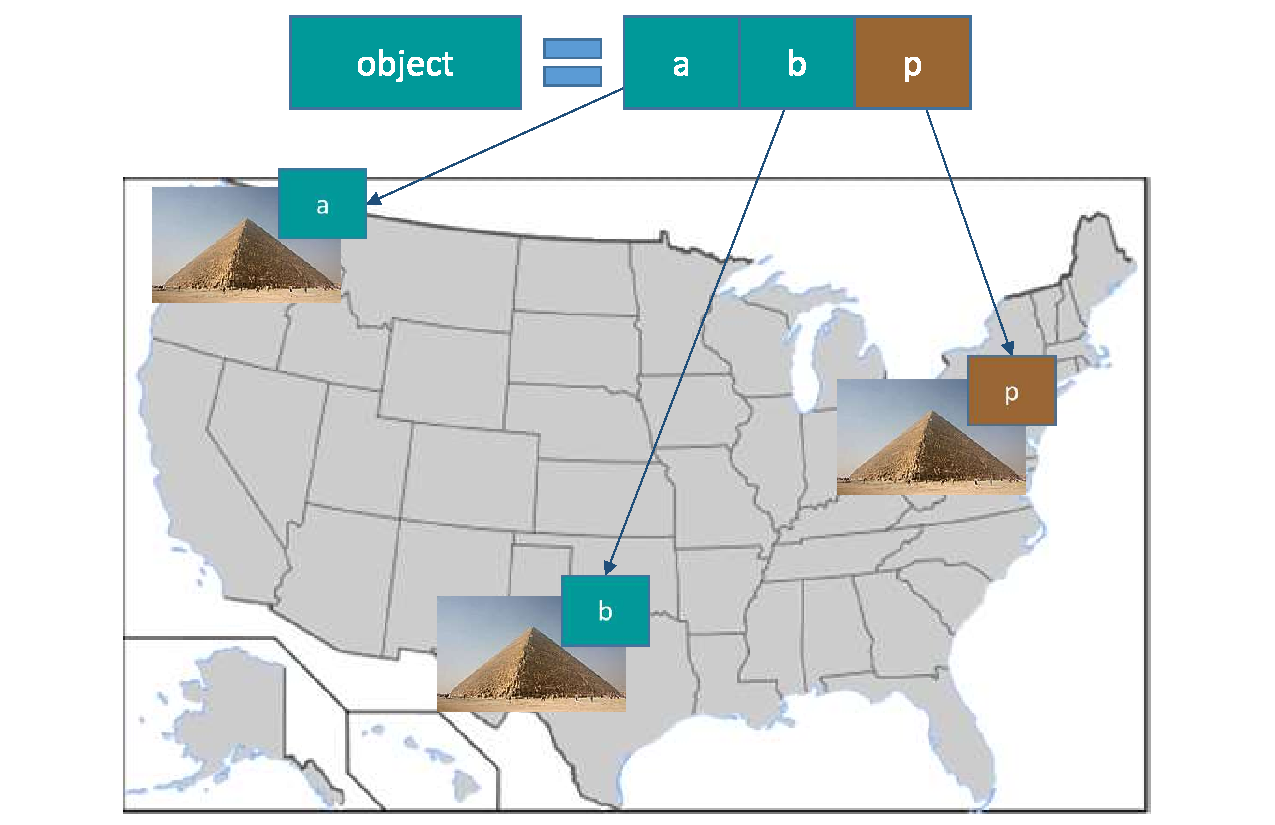
\includegraphics[width=0.5\textwidth]{images/giza_example_crop_fit}
\caption{Storing Object in Giza}
\label{fig:giza_example}
\end{figure}

Giza operates on top of existing cloud storage systems. It stores customer data
objects in cloud blob storage and the metadata of the objects in cloud table
storage. Figure~\ref{fig:giza_example} illustrates an exemplary flow of storing
an object of 4MB.
%Giza operates a number of {\em stateless} Giza nodes in every data center. Say a customer uses a Giza client (command line, library, or REST interface) to store a 4MB data object. The Giza client routes the {\em put} request to one of the Giza nodes in the data center closest to the customer.
Giza divides the data object into $2$ data fragments ($a$ and $b$) of 2MB each.
It then encodes the data fragments to generate a parity fragment $p$ of size
2MB. All the $3$ coded fragments (2 data and 1 parity) are stored in the blob
storage in 3 data centers. The metadata, consisting of the pointers to the
blobs, as well as versioning information, is stored in the table storage in the
same data centers.

\subsection{Challenges and Contributions}

The target workloads for Giza are large data objects in cloud drives, such as
Dropbox, Google Drive, and Microsoft OneDrive, etc. The common properties of
such workloads include: 1) large storage space consumption, 2) relatively cold
data, where a small percentage of data is occasionally accessed across large
volumes, 3) objects may be updated over time, but concurrent updates of the same
object is rare (albeit possible).

Given the target workloads, Giza optimizes for the common case, where there is
single writer and multiple readers. Giza strives to {\em make the common case
  fast}. In fact, the most optimized version of Giza achieves optimal latency,
which is single cross-DC round trip for both {\em put} and {\em get}.

On the other hand, Giza does handle concurrency properly, which could arise in
various situations. For instance, Giza tolerates data center failure. In the
event of a data center being temporarily unavailable (or simply slow), the
customers are able to continue to read and write data objects without much
impact. The unavailable (or slow) data center may miss updates, which could
potentially lead to conflict when they receive new updates again. Also, the
retry of {\em put} could be routed to a different data center and therefore
conflict with the previously unfinished {\em put}. Therefore, even though
concurrency is rare, it is crucial for Giza to {\em guarantee the rare case
  correct}. Indeed, Giza provides external consistency (linearizability).

Giza operates on top of existing cloud storage systems. 
%It stores data in cloud blob storage and metadata in cloud table storage across multiple data centers.
The blob and table storage within individual data centers operate independently.
Hence, while strongly consistent individually, the collection of the blob and
table storage across multiple data centers do not readily offer the desired
linearizability. The key technical challenge Giza addresses is how to achieve
optimal {\em put} with singler writer, while at the same time provide
linearizability under concurrency, over the collection of individual blob and
table storage across multiple data centers.

Towards this end, the paper makes the following contributions:
\begin{itemize}
    \item We have designed and implemented Giza, a strongly consistent,
      versioned object store that erasure codes objects across globally
      distributed data centers.
    \item Giza is fast in the common case: when there is no concurrency, Giza
      completes within single cross-DC round trip, which is optimal given the
      requirement to tolerate data center failure.
    \item Giza is correct when accessed concurrently: even with data center
      failure, Giza achieves external consistency.
    \item Giza employs well-known distributed algorithms, such as Paxos and Fast
      Paxos, in a novel way so that it operates on top of existing cloud storage
      systems.
    \item Giza is deployed in xxx data centers. Experimental results demonstrate
      that Giza achieves all our design goals. In particular, it is worth
      pointing out that Giza achieves much lower latency than naively adopting a
      globally consistent storage system, like CockroachDB (open source
      implementation of Google's Spanner).
\end{itemize}
